\Chapter{Abstract}

Die folgende Arbeit beschreibt die Struktur und den Entwicklungsprozess einer Implementierung
der RISC-V-ISA auf einem FPGA. Dabei wurden die logischen Bausteine in der
Hardwarebeschreibungssprache VHDL implementiert. Die Projektdauer beläuft sich auf zwei Semester, in denen
die vier Gruppenmitglieder simultan an den einzelnen Komponenten gearbeitet haben. Der Arbeit liegen selbstverst\"andlich der entstandene VHDL-Code sowie einige demonstrative Programme, die vom Prozessor korrekt ausgef\"uhrt werden k\"onnen, bei. Des Weiteren sind auch ein Assemblierer f\"ur das implementierte Instruction-Set sowie ein Simulator, der auf spezielle Umgebung der VHDL-Implementierung angepasst ist, enthalten.

\newpage

\Chapter{Projektablauf}

Zu Beginn des Projekts wurde eine Unterteilung der Anforderungen in einerseits ein Basisangebot sowie ein daran ankn\"upfendes Erweiterungsangebot vollzogen. W\"ahrend innerhalb des ersten Semesters vor allem der Fokus auf die Eingew\"ohnung in die Entwicklungsumgebung und Realisierung der Basisziele lag, sah die Planung f\"ur das zweite Semester eine eine Erweiterung des dann bereits lauff\"ahigen Prozessors um zus\"atzliche Module vor. 

\Section{Aufgabe}

<<<<<<< HEAD
Die Hauptaufgabe bestand darin, eine Implementierung eines funktionsf\"ahigen Prozessor auf Basis der \href{https://riscv.org/specifications/}{RISC-V Instruction Set Architecture} anzufertigen, welche auf dem zur Verf\"ugung gestellten Entwicklungsboard (\textit{Spartan-3A FPGA Starter Kit}) lauff\"ahig ist.
=======
Die Aufgabe bestand darin, einen funktionsf\"ahigen Prozessor auf Basis der RISC-V Instruction Set Architecture zu entwickeln, der auf dem FPGA des gegebenen Entwicklungsboards (\Externalname{Spartan-3A FPGA Starter Kit}) l\"auft.
>>>>>>> 5cd12b5445c8244076e68c39fe8701ec2b29a6a9
\begin{figure}[H]
	\centering
		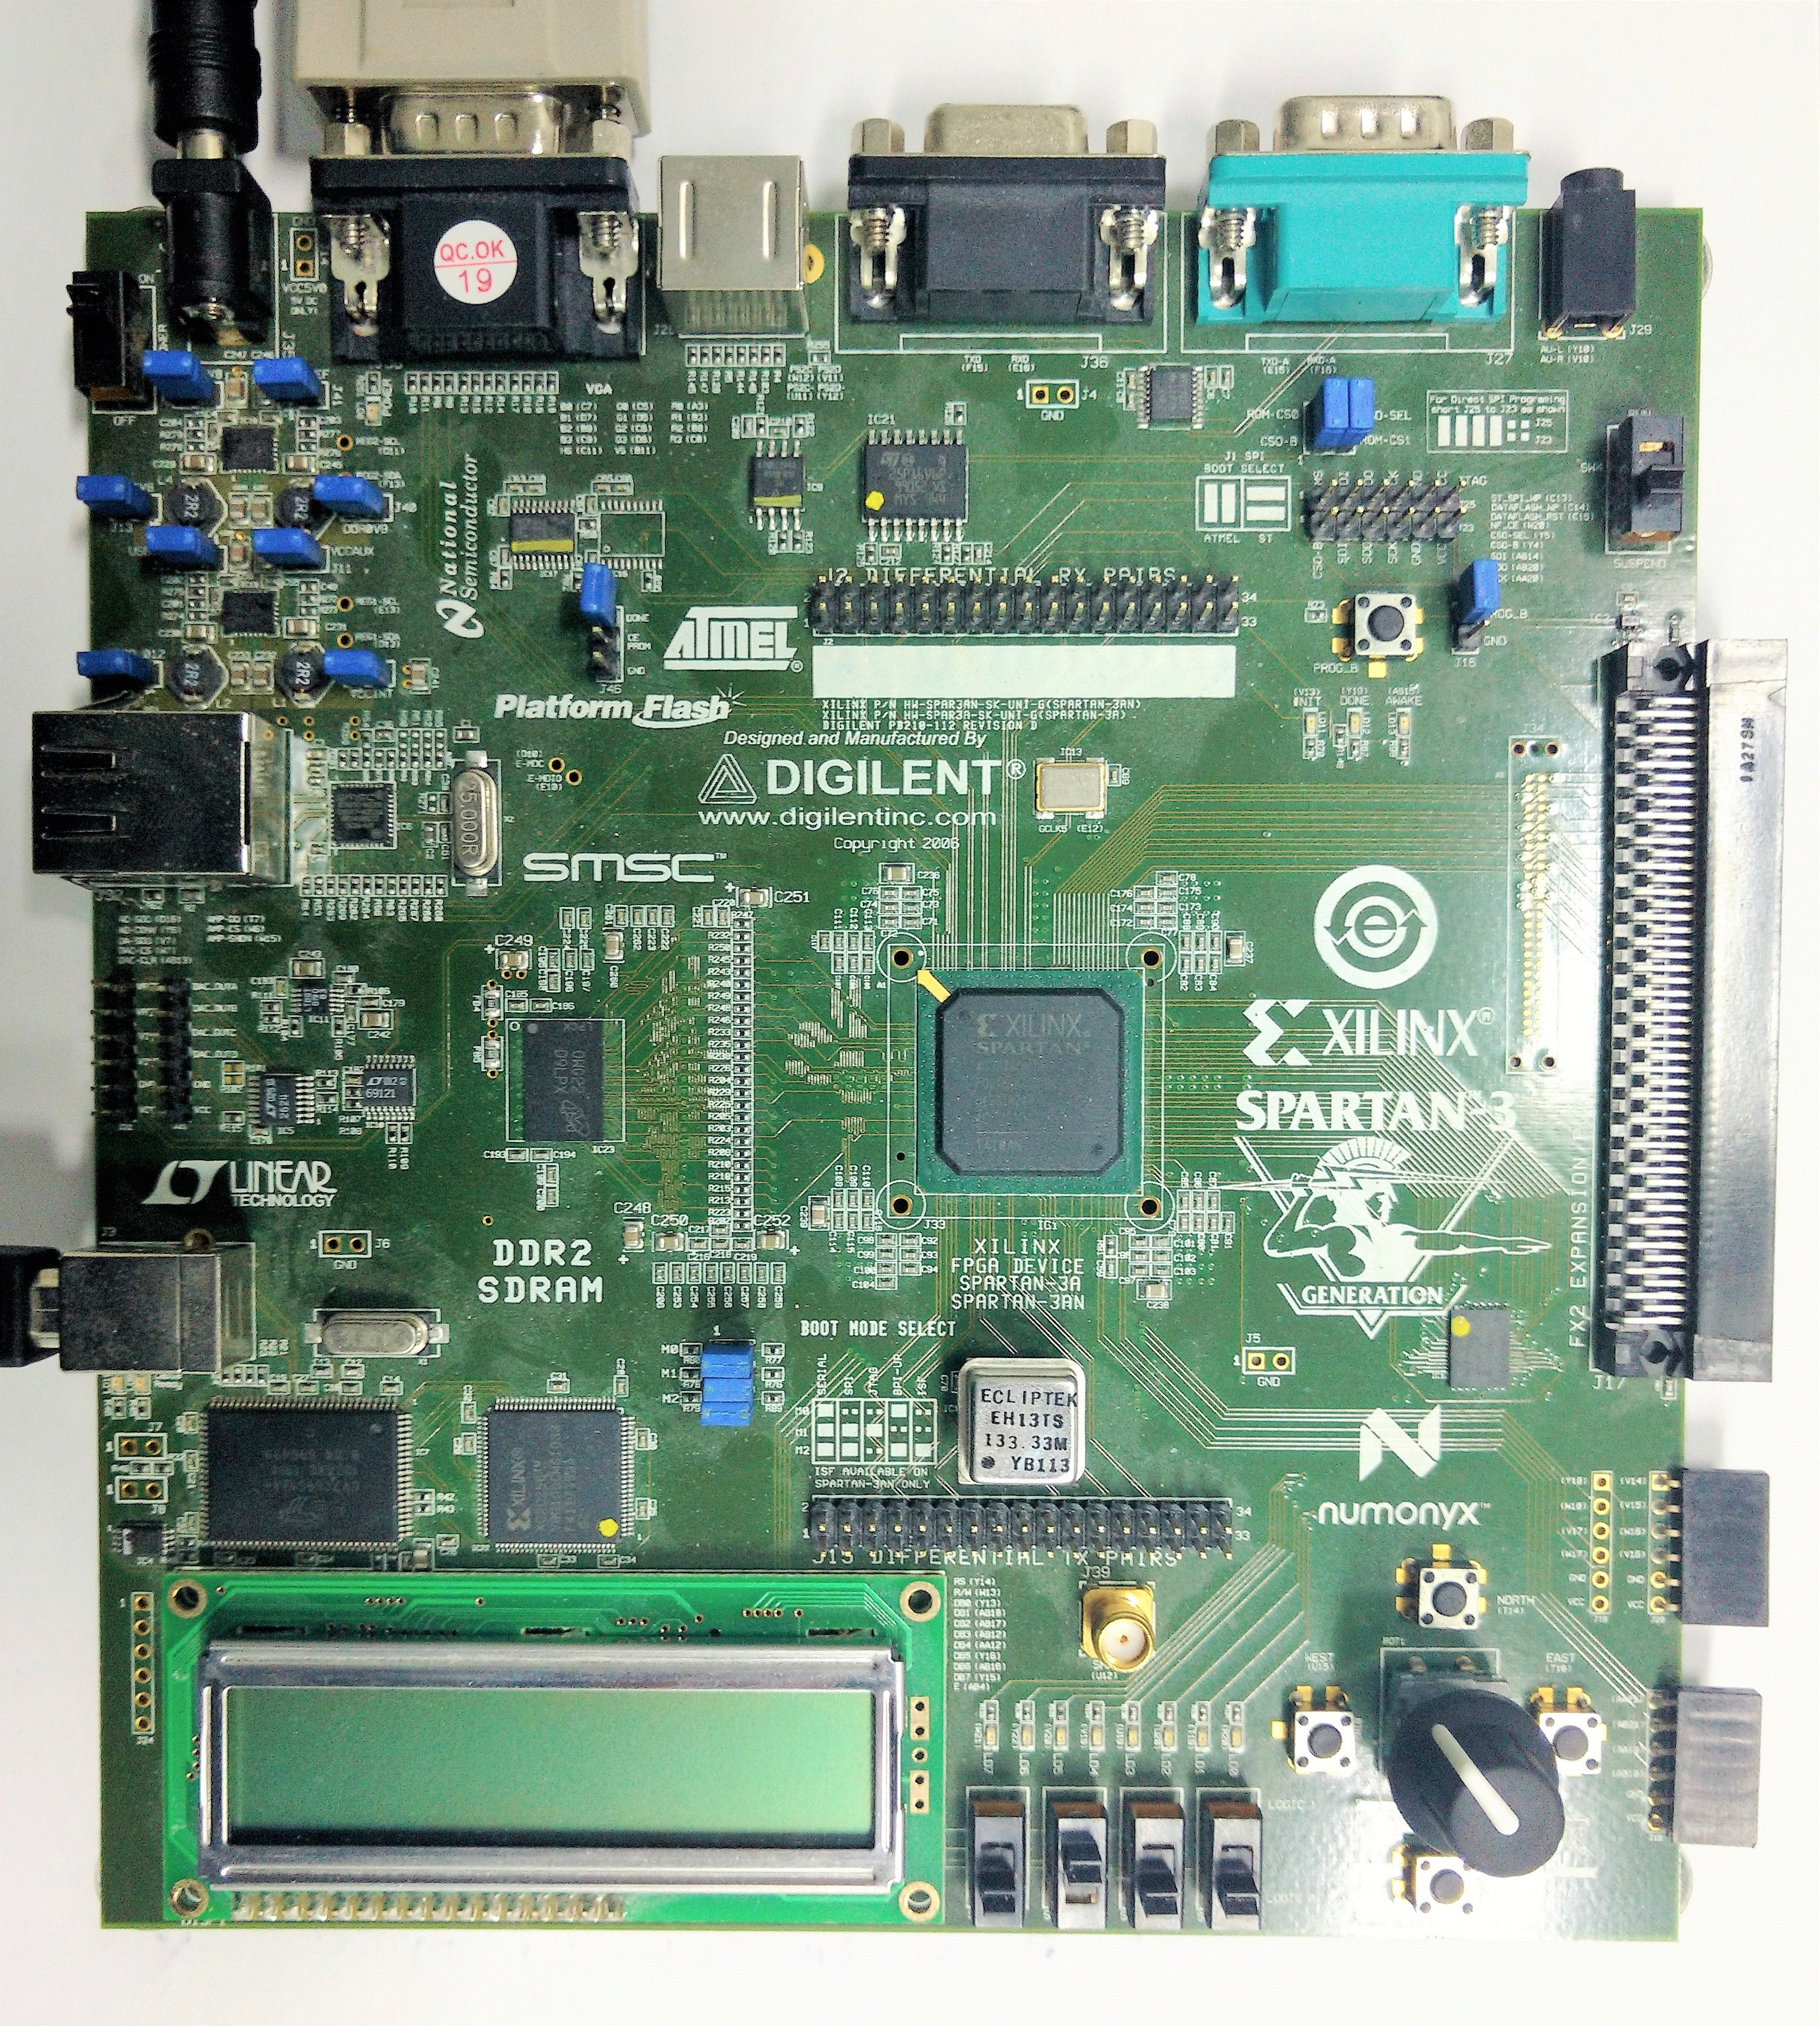
\includegraphics[width=0.3\textwidth]{Board.png}
	\caption[Entwicklungsboard]{Das verwendete Entwicklungsboard von oben, der FPGA liegt zentral}
	\label{fig:board}
\end{figure}
\Section{Basisziele}


<<<<<<< HEAD
Als Mindestanforderung sollte dabei die Kompatibilit\"at zur \textit{RV32I Base Integer Instruction Set} gew\"ahrleistet werden. Ausgenommen davon waren die speziell f\"ur Aspekte des Multithreadings auf Mehrkernprozessoren enthaltenen Befehle FENCE, FENCE.I, SCALL und SBREAK, da die geforderte Implementierung lediglich einen Rechenkern besitzen sollte.

Um die Funktionsf\"ahigkeit des Prozessors auch nach au{\ss}en hin sichtbar zu machen und damit einhergehend keine Black-Box Komponente zu entwickeln, sollte eine M\"oglichkeit zur Benutzerinteraktion \"uber geeignete, auf dem Entwicklungsboard vorhandene Bausteine wie etwa Schalter bestehen. Insbesondere zu Zwecken des Debuggings wurde auch eine grafische Ausgabe der internen Register \"uber die VGA-Schnittstelle zu einem angeschlossenen Monitor m\"oglich inkludiert.\footnote{Siehe dazu auch Pflichtenheft vom 02.06.16 bzw. 12.11.16}

\Section{Erweiterungsziele}


Die Modularit\"at der RISC-V ISA legt einige sinnvolle Erweiterungen nahe, darunter auch die \textit{RV32M Standard Extension for Integer Multiplication and Division}, welche Multiplikations- und Divisionsbefehle beinhaltet. Zudem sollte die rudiment\"are Ausgabe der internen Register um einen Textmodus erweitert werden, sodass mittels Memory-Mapping nun auch ASCII-Zeichen auf dem Monitor ausgegeben werden k\"onnen. Weiterhin wurde, um eine bessere Interaktion mit dem Programmierer zu erm\"oglichen, auch die Umsetzung einer seriellen Schnittstelle in den geplanten Erweiterungsrahmen miteinbezogen. Zuletzt stellt auch das Entwerfen eines demonstrativen Programms, genauer eines einfachen Spiels, ma\ss{}geblich einen Bestandteil des Erweiterungsangebots dar, sodass die endg\"ultige Implementierung adäquat pr\"asentieren sein sollte.
=======
Als Mindestanforderung sollte ein Prozessor mit Kompatibilit\"at zur \Externalname{RV32I Base Integer Instruction Set} implementiert werden. Ausgenommen davon sind die Befehle FENCE, FENCE.I, SCALL und SBREAK, da keine Hardwareunterst\"utzung f\"ur den Multitaskingbetrieb bereitgestellt werden soll.

Um die Funktionsf\"ahigkeit des Prozessors auch nach au{\ss}en sichtbar zu machen und keine Black-Box zu erstellen soll die M\"oglichkeit der Interaktion \"uber die Schnittstellen und Pins des Boards bestehen. Insbesondere soll zum Debugging eine grafische Registerausgabe \"uber den VGA-Port an einem Monitor m\"oglich sein.\footnote{Siehe dazu auch Pflichtenhefte vom 02.06.16 bzw. 12.11.16}

\Section{Erweiterungsziele}

Aufgrund der Modularit\"at von RISC-V bietet es sich an die Erweiterung \Externalname{RV32M Standard Extension for Integer Multiplication and Division} zu implementieren, welche Multiplikations- und Divisionsbefehle beinhaltet. Zudem soll die rudiment\"are Ausgabe um einen Textmodus erweitert werden, sodass mittels Memory-Mapping ASCII-Zeichen auf dem Monitor ausgegeben werden k\"onnen. Zum Demonstrieren der Funktionalit\"at soll au{\ss}erdem ein auf dem Prozessor lauff\"ahiges Spiel entwickelt werden. Um auch Daten\"ubertragung mit der Au{\ss}enwelt zu erm\"oglichen soll die serielle Schnittstelle genutzt werden.
>>>>>>> 5cd12b5445c8244076e68c39fe8701ec2b29a6a9

\Section{Projektablauf}
\Subsection{Chronologischer Verlauf}

Wie eingangs erw\"ahnt umfasste die Dauer des Praktikums zwei Semester, in denen im Allgemeinen drei verschiedene Implementierungsversionen angefertigt wurden.

<<<<<<< HEAD
\begin{figure}[H]
\begin{tabular}{|p{70pt}|p{60pt}|p{220pt}|p{110pt}|}
=======
\begin{table}[H]
\begin{tabular}{|p{50pt}|p{80pt}|p{220pt}|p{110pt}|}
>>>>>>> 5cd12b5445c8244076e68c39fe8701ec2b29a6a9
\hline
Versionsziele & Zeitraum                                   & Ziele                                                                            & davon nicht erreicht                          \\
\hline
Grundkonzept       & \mbox{April 2016 -} \mbox{Juni 2016}       & \begin{itemize}[noitemsep,topsep=0pt]
                                                       \item Pr\"ufung der Strukturierung des Prozessors in ALU, Leitwerk und MMU
                                                       \item Pr\"ufung der Arbeitsaufteilung
                                                       \item Entwickeln eines Verst\"andnisses f\"ur die Mechaniken der Tools
                                                       \item Ausf\"uhrbarkeit einiger grundlegender Befehle
                                                       \end{itemize}                                                                    &                                               \\
\hline
Endg\"ultige Ausarbeitung des Basisangebots      & \mbox{Juni 2016 -} \mbox{Sept. 2016}   & \begin{itemize}[noitemsep,topsep=0pt]
                                                       \item Implementierung der RV32I-Spezifikation
                                                       \item Lese- und Schreibzugriff auf den DDR2-SDRAM
                                                       \item Debugging-Ausgabe durch Darstellung der internen Register
                                                       \end{itemize}                                                                    & \begin{itemize}\item Lese- und Schreibzugriff auf den DDR2-SDRAM\end{itemize}     \\
\hline
Implementierung der Erweiterungsziele & \mbox{Sept. 2016 -} \mbox{Januar 2017} & \begin{itemize}[noitemsep,topsep=0pt]
                                                       \item Implementierung der RV32M-Spezifikation
                                                       \item Lese- und Schreibzugriff auf den DDR2-SDRAM
                                                       \item Erweiterung der Ausgabefunktionalit\"aten um einen Textmodus
                                                       \item Bereitstellung einer Benutzerschnittstelle durch Buttons, LEDs, \dots{} des Boards durch Memory-Mapped-I/O
                                                       \item Nutzbarkeit der seriellen Schnittstelle (UART)
                                                       \end{itemize}                                                                    & \begin{itemize}\item Nutzbarkeit der seriellen Schnittstelle (nur teilweise)\end{itemize}       \\
\hline
\end{tabular}
\caption{\"Ubersicht \"uber den Projektablauf}
\end{table}

<<<<<<< HEAD
Gem\"a\ss{} den vier Prinzipien der Von-Neumann-Architektur wurde die Implementierung grob in die Hauptkomponenten Leit-, Rechen-, Ein-/Ausgabewerk und Speicher gegliedert, was sich konkret in den drei Subkomponenten CU, ALU und MMU widerspiegelt. F\"ur jeden dieser Bausteine war durchg\"angig eine unabh\"angige Kleingruppe verantwortlich, wobei es trotzdem f\"ur sinnvoll erachtet wurde, w\"ochentliche Treffen zu Zwecken der Planung und Integration der Komponenten sowie zum Testen, zu veranschlagen. Entscheidungen von gr\"o\ss{}erer Tragweite, besonders im Hinblick auf generelle Designentscheidungen wurden meist im Plenum besprochen.

\Section{Verwendete Tools}

Das Projekt wurde in der Hardwarebeschreibungssprache VHDL implementiert, was sich darin begr\"undet, dass diese Themenkomplex der zugrundeliegenden Lehrveranstaltung war und die Gruppenmitglieder daher auf einem einigerma\ss{}en gleichwertigen Kenntnisstand waren.

Zur Entwicklung wurde haupts\"achlich die Entwicklungsumgebung Xilinx' \textit{ISE Project Navigator} in Version 14.7 verwendet. Diese erm\"oglichte einerseits das Editieren des VHDL-Codes und beinhaltete andererseits auch eine integrierte Toolchain, um den VHDL-Code in ein Programming-File zu übersetzen. Dieses wurde dann benutzt, um das Board zu programmieren. Der zus\"atzlich enthaltene \textit{Core Generator} wurde dabei verwendet, um einzelne Subkomponenten wie beispielsweise eine Divisionseinheit zu generieren.\\
=======
Da die Aufteilung eines Prozessors in Leitwerk, ALU und MMU nahe lag, wurde
f\"ur jede dieser Einheiten durchg\"angig eine Kleingruppe verantwortlich
gemacht. Dennoch wurde entschieden, dass ein Treffen pro Woche sinnvoll zum
Testen und Integrieren der einzelnen Einheiten ist. Es hat sich jedoch
herausgestellt, dass bei diesen Treffen meistens nur die Gruppen zweier
Einheiten ??????????????????

\Section{Verwendete Tools}
Das Projekt wurde in VHDL implementiert, da s\"amtliche Programmierer ausschlie{\ss}lich in dieser Hardwarebeschreibungssprache gute Kenntnisse hatten.\\
Zur Entwicklung wurde haupts\"achlich Xilinx' \Externalname{ISE Project Navigator} in Version 14.7 verwendet. Dieser diente zugleich als Editor f\"ur den VHDL-Code und auch als Werkzeug um daraus die Programming-Files, mit welchen das FPGA beschrieben wird, zu generieren. Der integrierte \Externalname{Core Generator} wurde dabei benutzt um einzelne Module zu erstellen.\\
>>>>>>> 5cd12b5445c8244076e68c39fe8701ec2b29a6a9
\begin{figure}[H]
	\centering
		\includegraphics[width=1.0\textwidth]{ISE.png}
	\caption[\Externalname{ISE Project Navigator}]{Der Xilinx \Externalname{ISE Project Navigator}}
	\label{fig:tool}
\end{figure}
<<<<<<< HEAD
Mittels des Tools \textit{impact}, welches ebenfalls vom Anbieter der Entwicklungsumgebung Xilinx stammt, konnte in Kombination mit einem \textit{Cable-Server} das Board mit \"uber USB gem\"a{\ss} den erstellten Programming-Files beschrieben werden.\\
Zur Versionsverwaltung wurde dabei auf ein \textit{Git- Repository} gesetzt.\\ 

Um sich die doch recht umfassende Arbeit des Assemblierens eines Programms nicht h\"andisch erledigen zu m\"ussen, wurde, wie sp\"ater genauer erl\"autert wird, ein automatischer Assemblierer in der Scriptsprache Python entwickelt.
Um nicht jedes zu testende Programm per Hand assemblieren zu m\"ussen wurde ein Assemblierer auf Python-Basis erstellt.\\
Da die Generierung eines Programming-Files und das anschlie{\ss}ende Beschreiben des FPGAs nichtsdestotrotz jedes Mal mehrere Minuten in Anspruch genommen hatte, wurden entsprechende Simulatoren verwendet. Zur Verifikation des VHDL-Codes beispielsweise wurde so das Tool \textit{GHDL} in Kombination mit \textit{GTKWave} benutzt. Auch zum Testen der Assemblerprogramme wurde ein Simulator auf Python-Basis, der die Umgebung des Boards emuliert, entworfen und in den Arbeitsprozess mit eingebunden.
=======
Mittels Xilinx' \Externalname{impact} in Kombination mit dem \Externalname{Cable-Server} wurde das Board dann \"uber USB gem\"a{\ss} den Programming-Files beschrieben.\\
Zur Versionsverwaltung wurde dabei auf ein \Externalname{Github Repository} gesetzt.\\ 
Um nicht jedes zu testende Programm per Hand assemblieren zu m\"ussen wurde ein Assemblierer auf \Externalname{Python}-Basis erstellt.\\
Da die Generierung eines Programming-Files mit anschlie{\ss}endem Beschreiben des FPGAs selbst dann noch jedes Mal mehrere Minuten in Anspruch nimmt, wurden zum schnelleren Testen Simulatoren verwendet. Um den VHDL-Code zu verifizieren wurde so \Externalname{GHDL} in Kombination mit \Externalname{GTKWave} verwendet. Auch zur Assemblerprogrammierung wurde ein Simulator mitsamt Textausgabe entwickelt um schneller debuggen zu k\"onnen.
>>>>>>> 5cd12b5445c8244076e68c39fe8701ec2b29a6a9
